\section{Durchführung}
\label{sec:Durchführung}

Der Versuchsaufbau ist in der folgenden Abbildung dargestellt
\begin{figure}
    \centering
    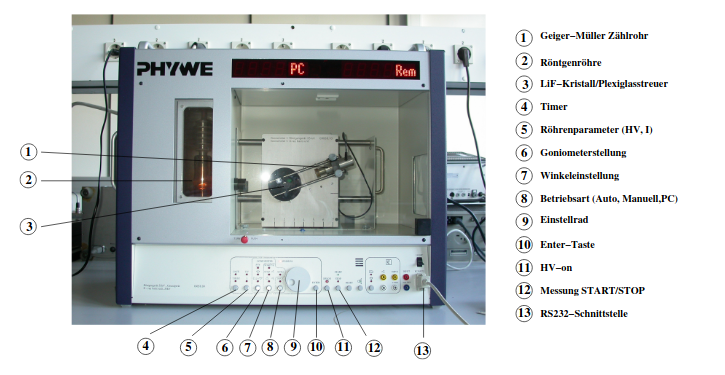
\includegraphics{Röntgenröhre.png}
    \caption{Experimenteller Versuchsaufbau}
    \label{fig:hex}
  \end{figure}
Im Wesentlichen besteht er aus einer Röntgenröhre, einem LiF-Kristall und einem 
Geiger-Müller-Zählrohr. 
\\
\\
Zunächst wird zur Überprüfung der Braggbedingung der LiF-Kristall auf einen festen Winkel eingestellt
und der Winkel des Geiger-Müller-Zählrohrs variiert. Im nächsten Schritt wird nun das 
Emissionsspektrum gemessen.\\
Im Anschluss werden verschiedene Absorber vor dem Geiger-Müller-Zählrohr installiert und die 
Absorptionsspektren aufgenommen.